

\section{authentication overflow 1}
\label{sec:auth_overflow1}
Bei diesem Angriff geht es darum, einen Buffer-overflow zu provozieren. Dies ist möglich, weil in der Methode strcpy aufgerufen wird, um das übergebene Passwort in den Buffer zu kopieren. Diese Methode überpfrüft nicht die Länge des übergebenen Passwortes, wodurch es vorkommen kann, dass mehr in den Buffer kopiert wird, als der Buffer groß ist. Dabei werden dann andere lokale Variablen, der Basepointer und die Rücksprungadresse überschrieben. 
Bei diesem Angriff ist es das Ziel die lokle variable zu überschreiben, in der das Flag für das Passwort gespeichert wird. Falls das Passwort richtig ist, dann wird das Flag auf den Wert 0x30303030 gesetzt. Falls das Passwort falsch ist, bleibt der Standartwert erhalten. Das lässt sich auch gut im Programmcode erkennen.

%todo hier bild von programmcode

Diesen Standartwert überschreiben wir durch den Buffer-overflow. Das lässt sich mit dem folgenden Befehl durchführen:\\
\begin{center}
    run \$(perl -e 'print "0"x2112')
\end{center}

Anschließend erhalten wir die Meldung, dass wir nun die Rechte bekommen haben. 

% hier Bild, dass wir Rechte haben

Mit diesen Rechten ist es möglich das Flag auszulesen.

Der Angriff ist ist im GDB nachvollziehbar. In diesem ist es möglich, Breakpoints zu setzen und sich den Inhalt des Stacks und der Register anzeigen zu lassen

%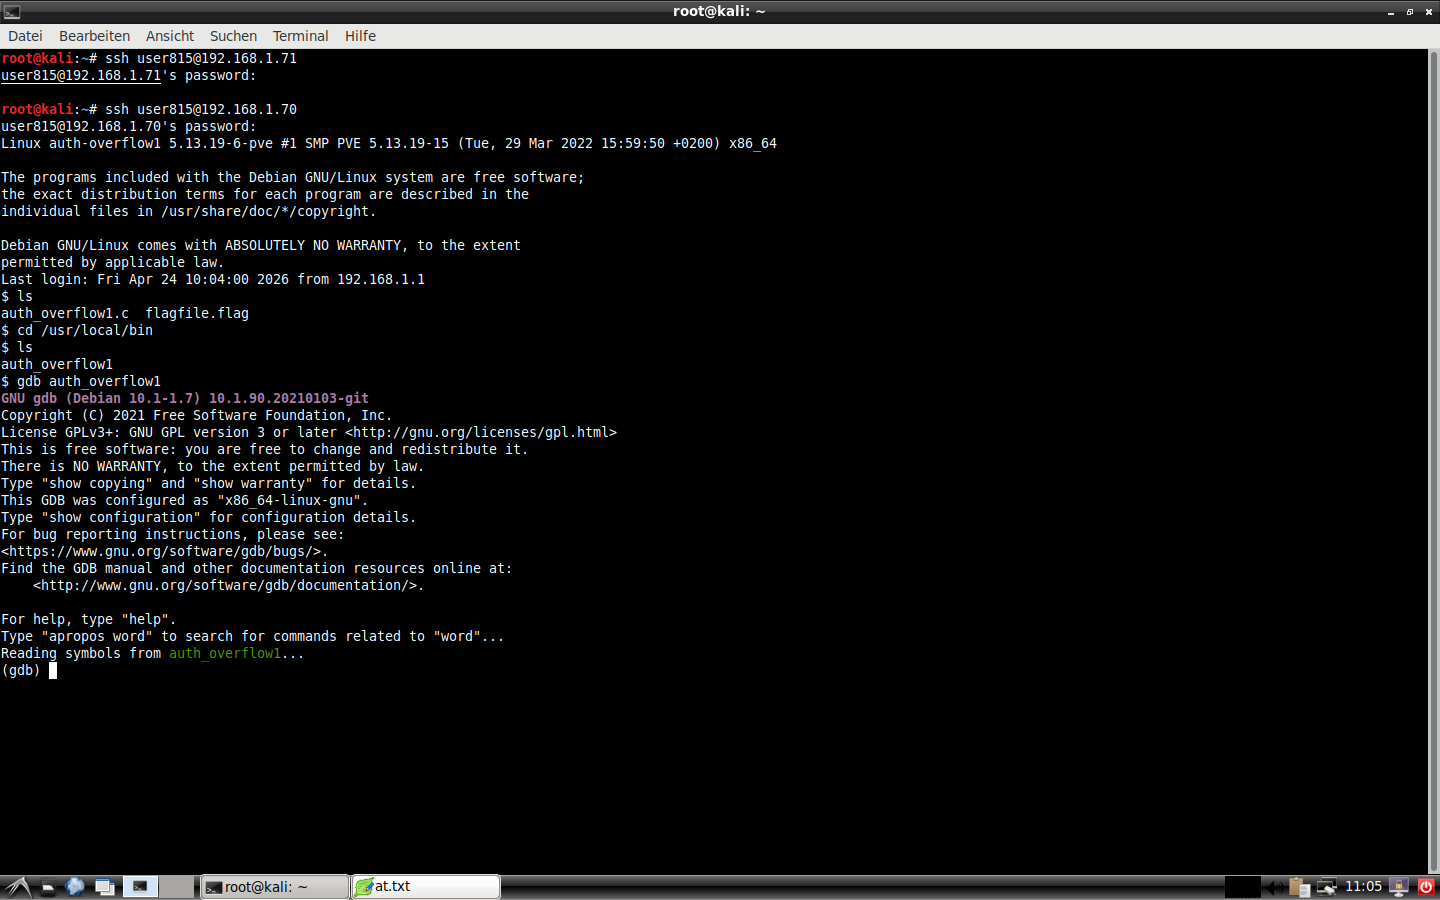
\includegraphics[width=\textwidth]{img/fingeruebungen/fingeruebung1_ssh_to_gdb.png}
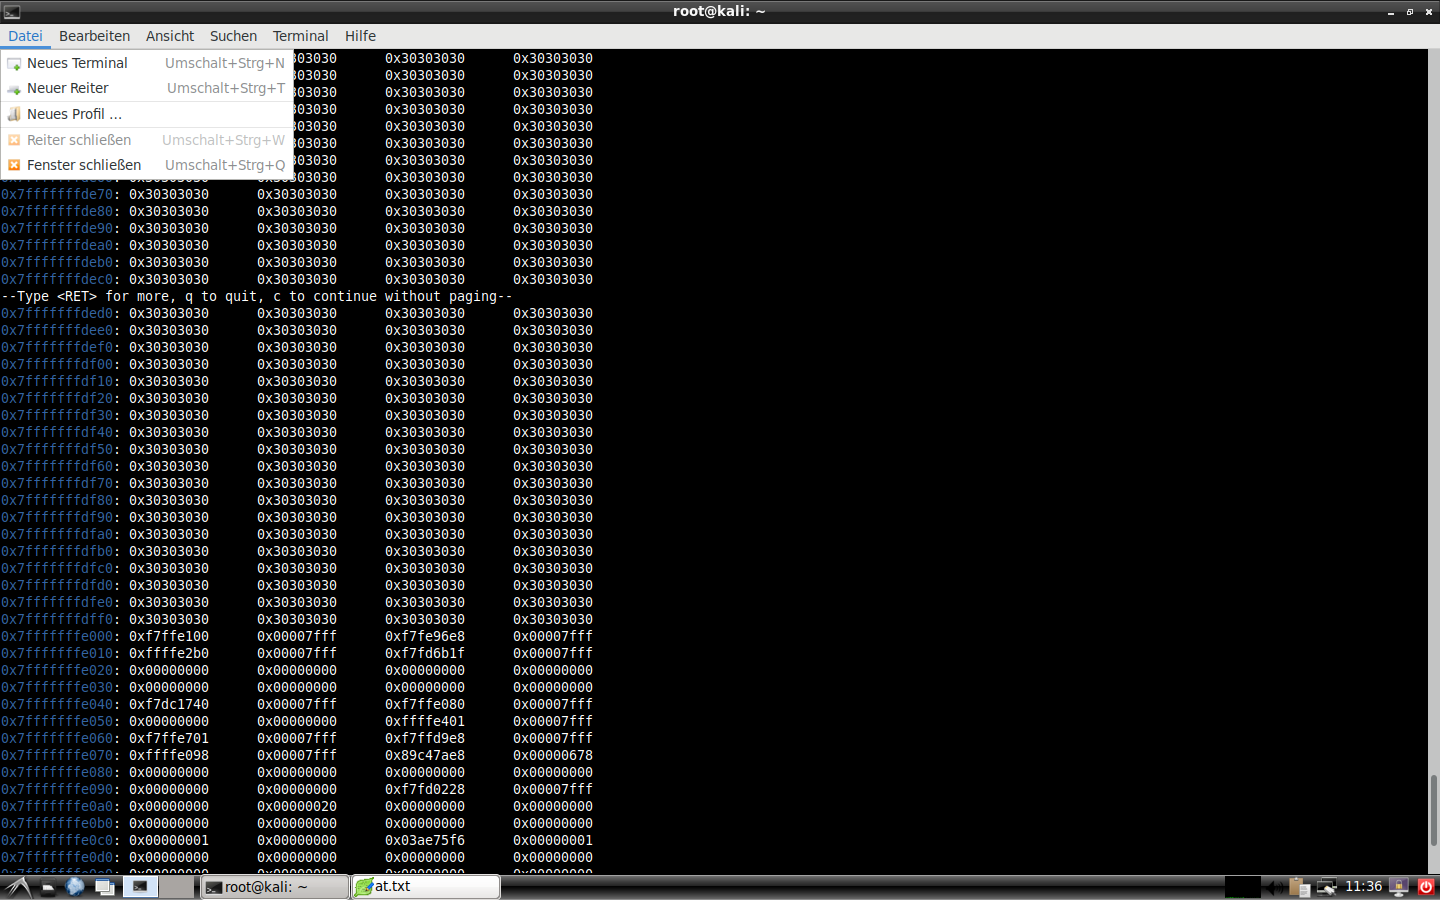
\includegraphics[width=\textwidth]{img/fingeruebungen/stack1.png}
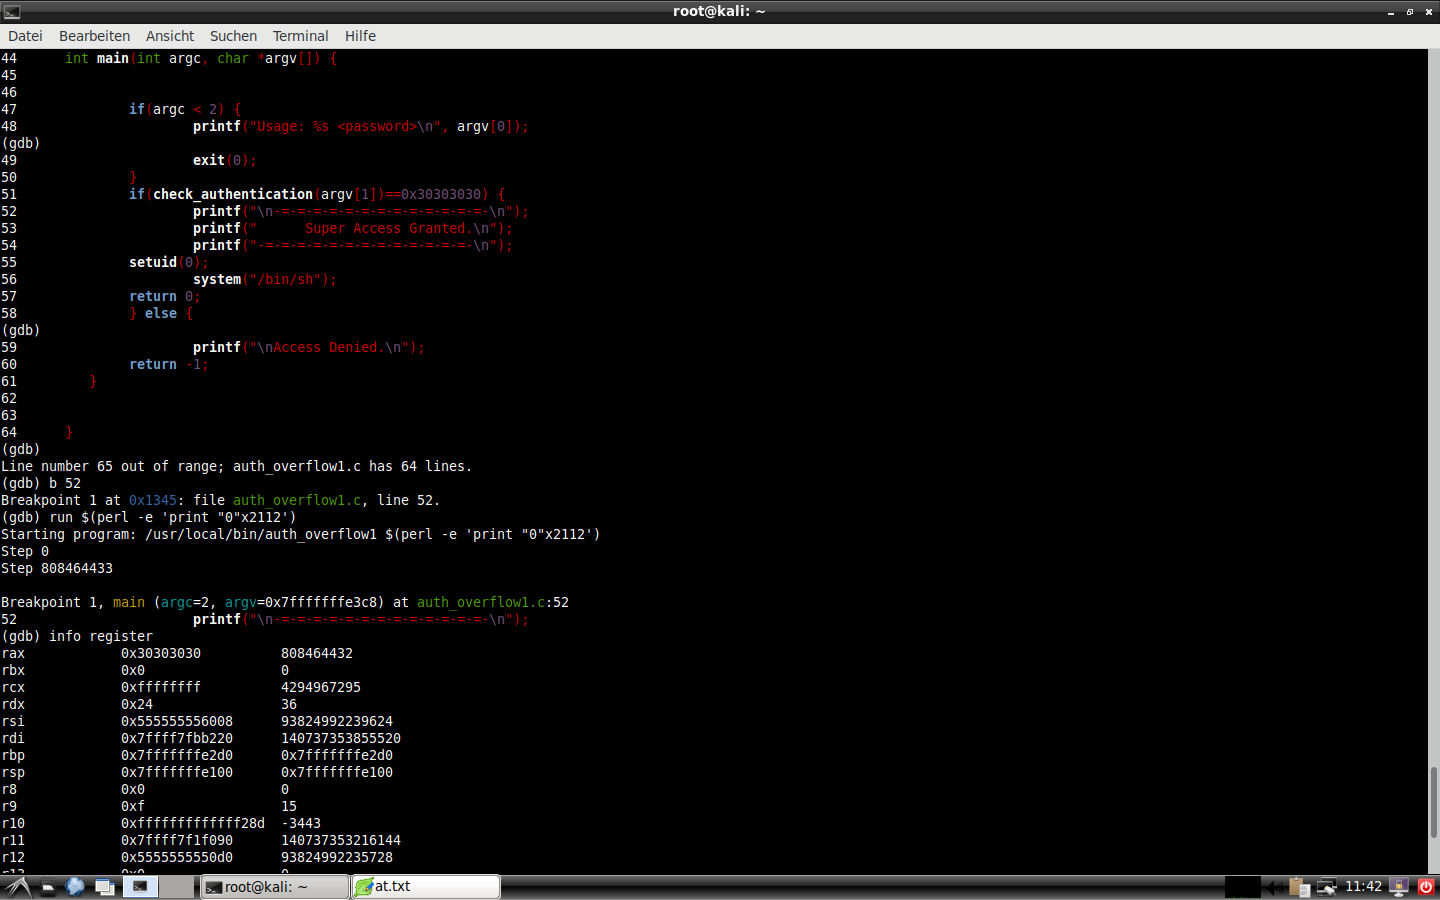
\includegraphics[width=\textwidth]{img/fingeruebungen/return_value_1.png}
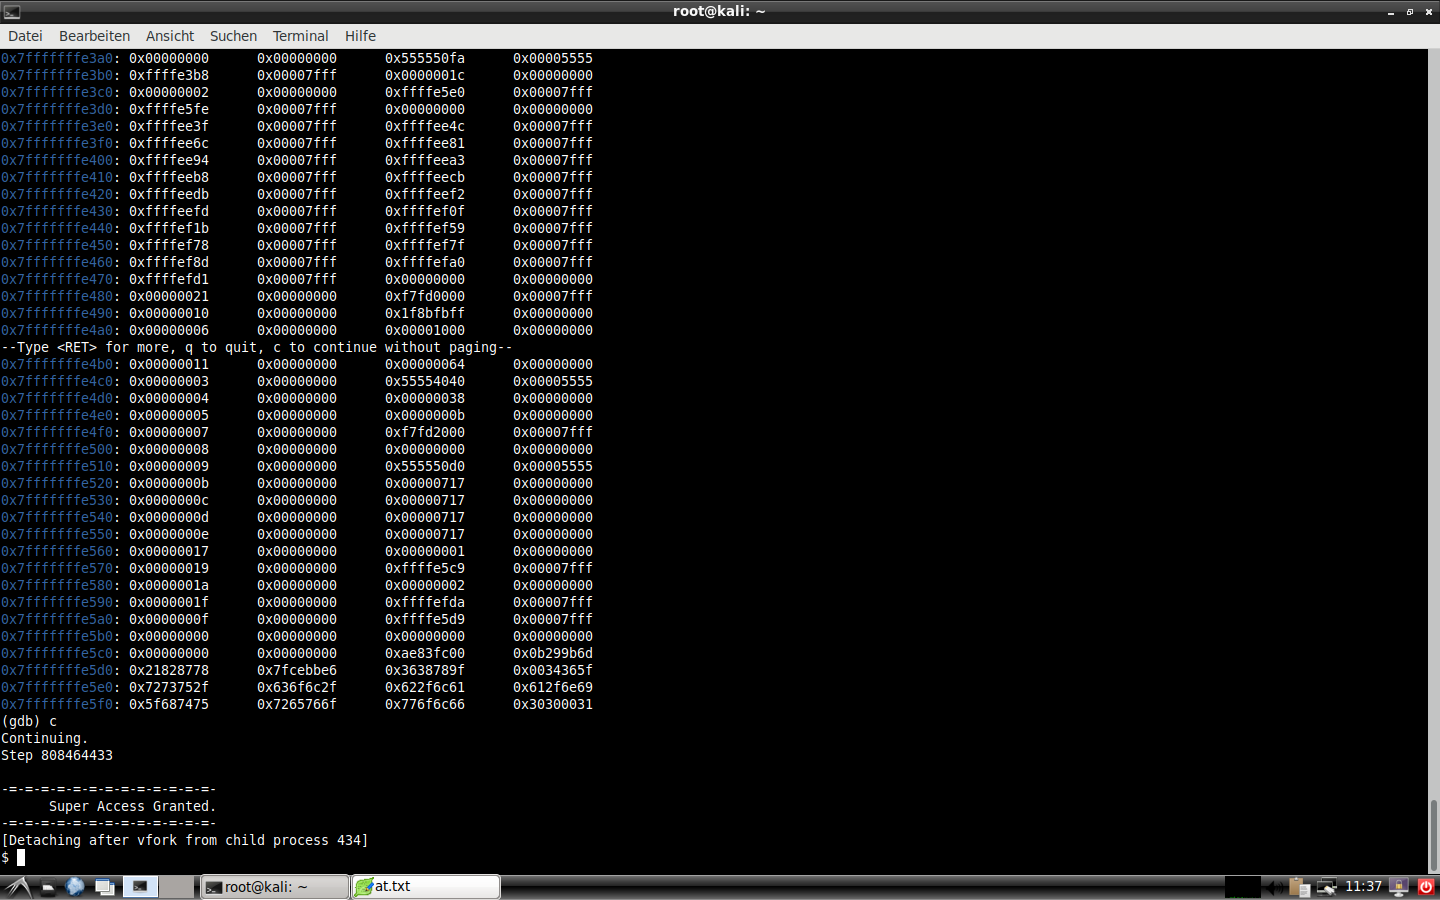
\includegraphics[width=\textwidth]{img/fingeruebungen/super_access_granted1.png}

\section{authentication overflow 2}
Wie auch bei \autoref{sec:auth_overflow1} wird ein Buffer-Overflow auf dem Stack provoziert. Diesmal wird aber nicht der Return-Wert überschrieben, sondern die Das lässt sich mit dem folgenden Befehl durchführen:\\
\begin{center}
    (Befehl)
\end{center}
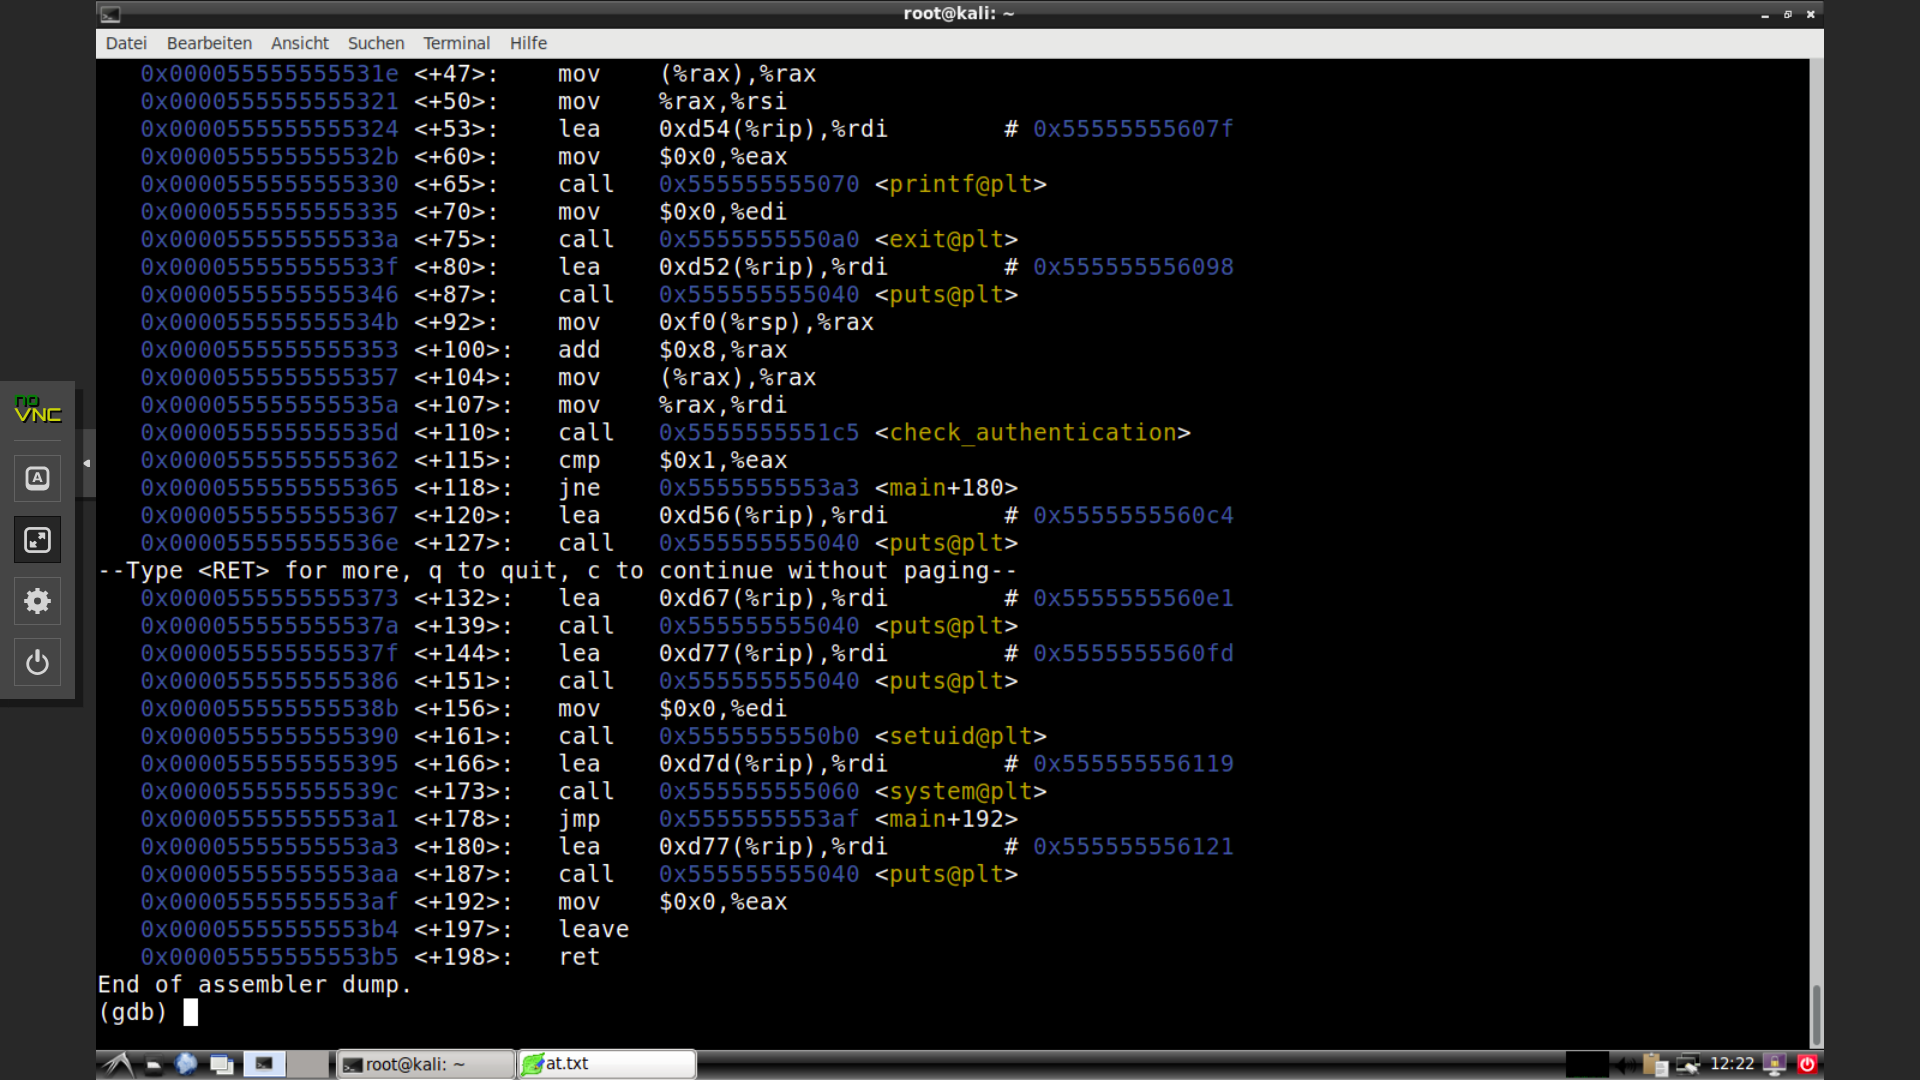
\includegraphics[width=\textwidth]{img/fingeruebungen/disass_main_2.png}
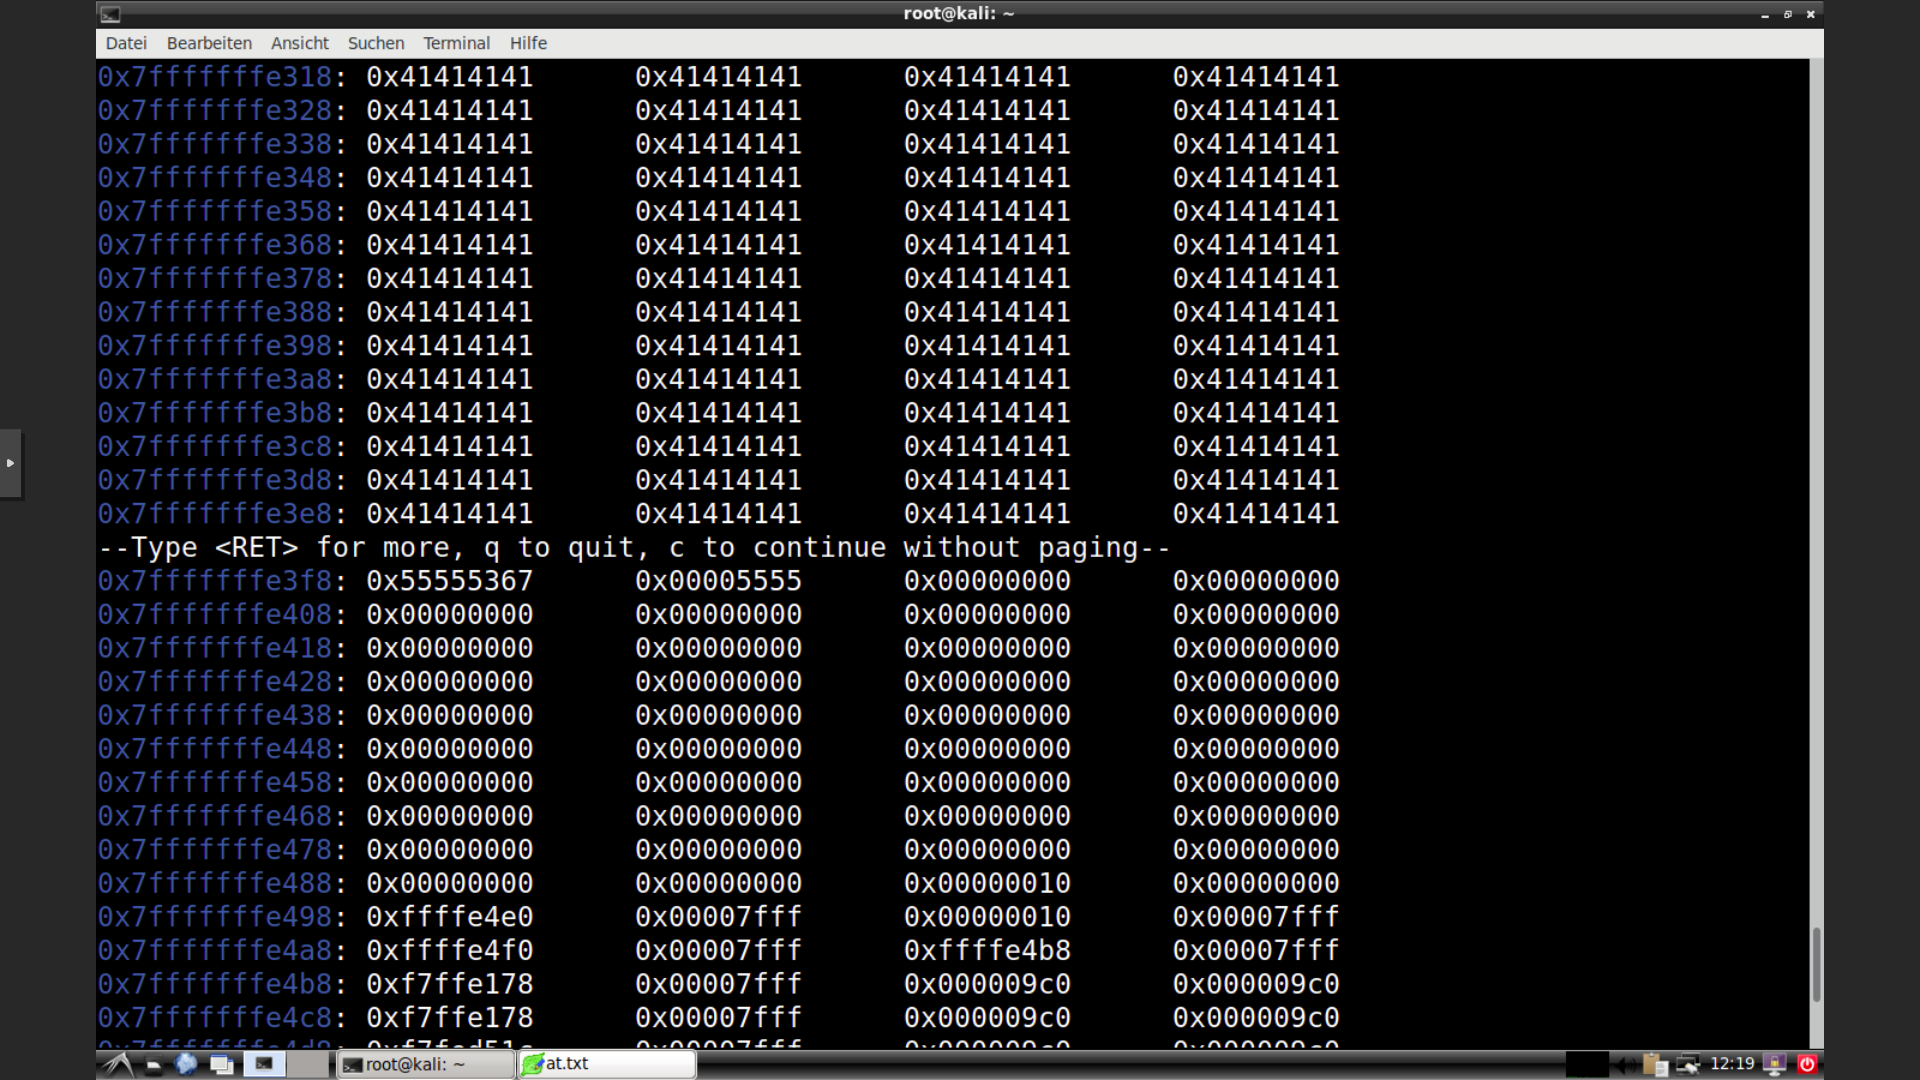
\includegraphics[width=\textwidth]{img/fingeruebungen/success_stack_2.png}
%TODO: Access Granted

\section{Probleme}
\begin{itemize}
    \item Lösung innerhalb des Gnu-Debuggers führte nicht zu Root-Rechten
    \item Rücksprung-Adresse wurde falsch gewählt
    \item Es wurde nicht genug überschrieben, wodurch bereits beim Basepointer aufgehört wurde und die Rücksprungadresse nicht überschrieben wurde.
    \item Die Nullterminierung verursachte Probleme. Lösung war, mehr 5en reinzuschreiben.
\end{itemize}

\section{Rechte}
Ursprünglich hatten wir normale User-Rechte. Nach dem Exploid haben wir Root-Rechte, wodurch wir die lesegeschützte Datei lesen können.


\section{Typ}
Es handelt sich um einen Stack-based-Buffer-Overflow.